\subsubsection{Servizi}

\subsubsubsection{AuthenicationService} \label{AuthenticationService}
\begin{figure}[H]
    \centering
    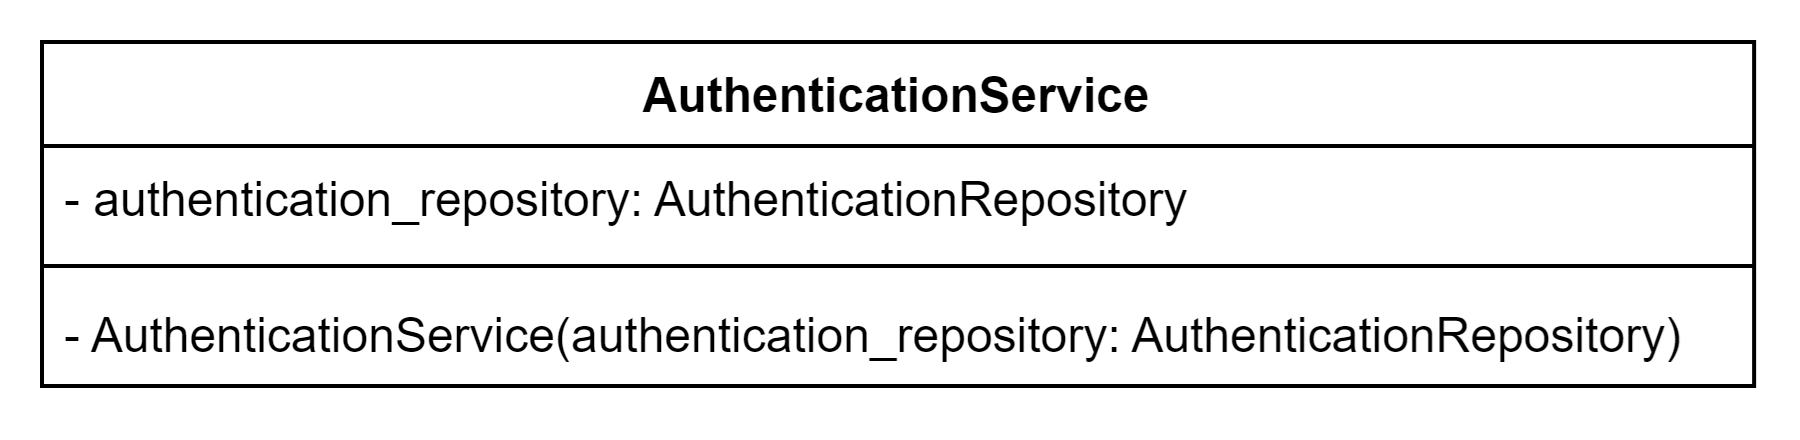
\includegraphics[width=0.7\textwidth]{assets/Backend/authentication_service.png}
    \caption{Diagramma della classe AuthenticationService}
  \end{figure}
\begin{itemize}
    \item \textbf{Descrizione}: AuthenticationService implementa il caso d'uso di autenticazione;
    \item \textbf{Interfaccia implementata}: \hyperref[AuthenticationUseCase]{AuthenticationUseCase};
    \item \textbf{Attributi}:
    \begin{itemize}
        \item \texttt{authentication\_repository}: istanza della classe utilizzata per gestire gli utenti nel sistema.
    \end{itemize}
    \item \textbf{Metodi}: 
    \begin{itemize}
        \item \texttt{+ login(username: string, password: string)}: autentica un utente basandosi sullo username e sulla password forniti. Restituisce un oggetto di risposta che include un messaggio di stato e, in caso di successo, il token di autenticazione.
    \end{itemize}
    \item \textbf{Dipendenze}:
    \begin{itemize}
        \item AuthenticationRepository.
    \end{itemize}
\end{itemize}  

\subsubsubsection{DictionaryService} \label{DictionaryService}
\begin{figure}[H]
    \centering
    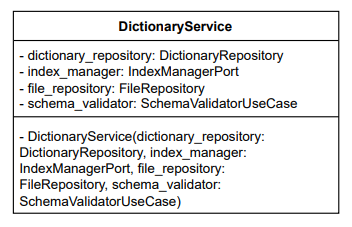
\includegraphics[width=0.8\textwidth]{assets/Backend/dictionary_service.png}
    \caption{Rappresentazione della classe DictionaryService}
  \end{figure}
\begin{itemize}
    \item \textbf{Descrizione}: DictionaryService è responsabile della gestione dei \glossario{dizionari dati};
    \item \textbf{Interfaccia implementata}: \hyperref[DictionaryUseCase]{DictionaryUseCase};
    \item \textbf{Attributi}:
    \begin{itemize}
        \item \texttt{dictionary\_repository}: istanza della classe utilizzata per gestire i dati dei dizionari;
        \item \texttt{index\_manager}: istanza del gestore degli \glossario{indici};
        \item \texttt{file\_repository}: istanza del gestore dei file;
        \item \texttt{schema\_validator}: istanza della classe utilizzata per validare lo schema dei dizionari.
    \end{itemize}
    \item \textbf{Metodi}:
    \begin{itemize}
        \item \texttt{+ get\_dictionary\_list()}: recupera la lista di tutti i dizionari;
        \item \texttt{+ get\_dictionary\_by\_id(id: integer)}: recupera un dizionario tramite il suo id;
        \item \texttt{+ get\_dictionary\_file(id: integer)}: recupera il percorso del file tramite il suo id;
        \item \texttt{+ get\_dictionary\_preview(id: integer)}: recupera l'anteprima del dizionario tramite il suo id;
        \item \texttt{+ create\_dictionary(dictionary: DictionaryDto, content: string)}: crea un nuovo dizionario e salva il file associato;
        \item \texttt{+ update\_dictionary\_metadata(id: integer, dictionary: DictionaryDto)}: aggiorna i metadati di un dizionario esistente;
        \item \texttt{+ update\_dictionary\_file(id: integer, content: string)}: aggiorna il file di un dizionario esistente;
        \item \texttt{+ delete\_dictionary(id: integer)}: elimina un dizionario esistente, inclusi il file e l'indice associati;
        \item \texttt{- file\_size\_checker(content: string)}: controlla se la dimensione del file rientra nei limiti consentiti.
    \end{itemize}
    \item \textbf{Dipendenze}:
    \begin{itemize}
        \item DictionaryRepository;
        \item IndexManagerPort;
        \item FileRepository;
        \item SchemaValidatorUseCase.
    \end{itemize}
\end{itemize}

\subsubsubsection{PromptManagerService} \label{PromptManagementService}
\begin{figure}[H]
    \centering
    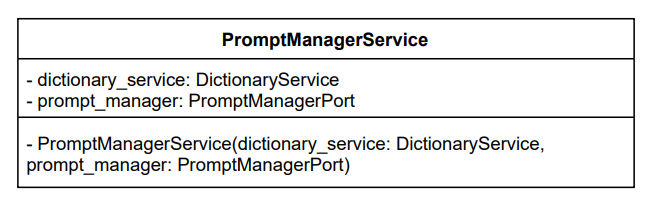
\includegraphics[width=0.8\textwidth]{assets/Backend/prompt_manager_service.png}
    \caption{Rappresentazione della classe PromptManagerService}
  \end{figure}
\begin{itemize}
    \item \textbf{Descrizione}: PromptManagerService si occupa di gestire le operazioni relative alla generazione di \glossario{prompt};
    \item \textbf{Interfaccia implementata}: \hyperref[PromptUseCase]{PromptUseCase};
    \item \textbf{Attributi}:
    \begin{itemize}
        \item \texttt{dictionary\_service}: istanza del servizio di gestione dei dizionari;
        \item \texttt{prompt\_manager}: istanza del gestore dei prompt.
    \end{itemize}
    \item \textbf{Metodi}:
    \begin{itemize}
        \item \texttt{+ generate\_prompt(dictionary\_id: integer, query: string, dbms: string,\\ language: string)}: genera un prompt a partire da una richiesta, un dizionario, una lingua e un \glossario{DBMS};
        \item \texttt{+ generate\_prompt\_with\_debug(dictionary\_id: integer, query: string, \\ dbms: string, language: string)}: genera un prompt con informazioni di \glossario{debug} relative ad esso;
        \item \texttt{- generate\_prompt(dictionary\_id: integer, query: string, dbms: string,\\ language: string, log: bool)}: metodo interno per attivare la generazione del prompt utilizzando il prompt manager.
    \end{itemize}
    \item \textbf{Dipendenze}:
    \begin{itemize}
        \item DictionaryService;
        \item PromptManagerPort.
    \end{itemize}
\end{itemize}  